\chapter{Testing and Evaluation}
The following chapter will cover the steps taken for evaluating the model in terms of performance and accuracy. A number of performance measures are used for determining how well the model handles data that it has not been trained with. These include training evaluation, testing with the testing data and inference with new data.

\section{Training Evaluation}
During the training of the model, a number of metrics were recorded for evaluation. The loss (often referred to as the cost function) is calculated by measuring the difference of the actual label value minues predicted output (See below).
 
\[H_{y’} (y) := - \sum_{i} y_{i}’ \log (y_i)\]

This value can be seen as a measure of how well the model is training. The closer the loss is to zero, the more accurate the model is at classifying. As seen in Figure \ref{loss}, the initially loss for the first epoch was approximately 185. This value decreased gradually throughout the training of the network, getting closer to 0.

\begin{figure}[ht]
	\begin{center}
		\advance\leftskip-3cm
		\advance\rightskip-3cm
		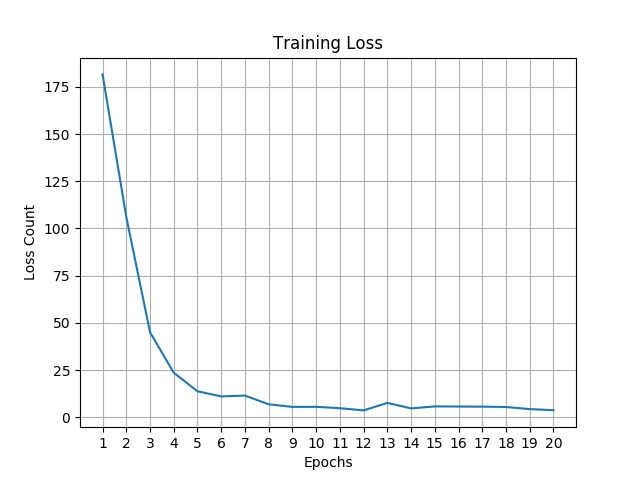
\includegraphics[keepaspectratio=true,scale=0.7]{__resources/Results/loss.jpg}
		\caption{Loss Function Values}
		\label{loss}
	\end{center}
\end{figure}

\newpage

The second training measurement taken into account was the accuracy throughout each step in training. This is measure by the adding the true positive with the true negative results, and dividing the sum by the total number of samples (See equation 6.1.1). It is said that using accuracy is not a desirable method of measuring performance, as it can give misleading results if there is a high class imbalance, which is not problem in our case as it was made sure that each class was represented equally.

\begin{equation}\label{eq:ac}
Accuracy = 
\frac{
True positive + Σ True negative
}{
Total population
}
\end{equation}

Intuitively, it is desired to have the highest accuracy possible. As can be seen in Figure \ref{acc}, the model performed rather well as it reached a high accuracy of approximately 98 percent and plateaued for the remainder of training.
\begin{figure}[ht]
	\begin{center}
		\advance\leftskip-3cm
		\advance\rightskip-3cm
		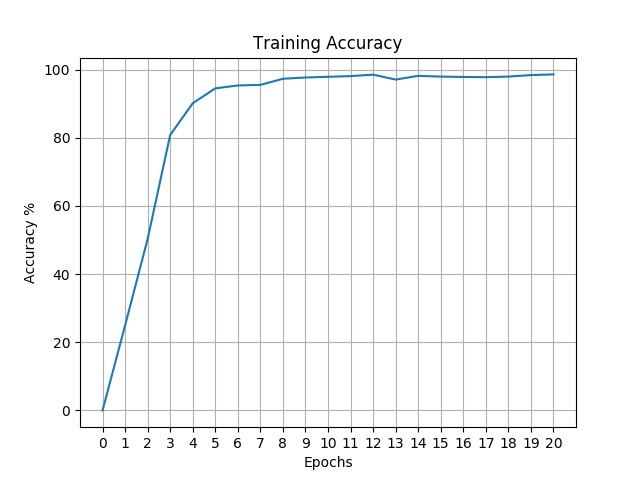
\includegraphics[keepaspectratio=true,scale=0.7]{__resources/Results/accuracy.jpg}
		\caption{Accuracy Values}
		\label{acc}
	\end{center}
\end{figure}

\newpage
\section{Testing Model with Testing Data}
As stated in the implementation chapter, the dataset was split into training and testing sets. out of the 1750 images for each class, 1400 of them were used for training, and the remaining 350 were used for testing the models performance. A python evaluation script was used for loading each set of classes individually and feed them to the trained model. Upon inspection, the network performs very well with most of the images being classified correctly, apart from the neutral class, which can be seen in Figure \ref{conf}.
\begin{figure}[ht]
	\begin{center}
		\advance\leftskip-3cm
		\advance\rightskip-3cm
		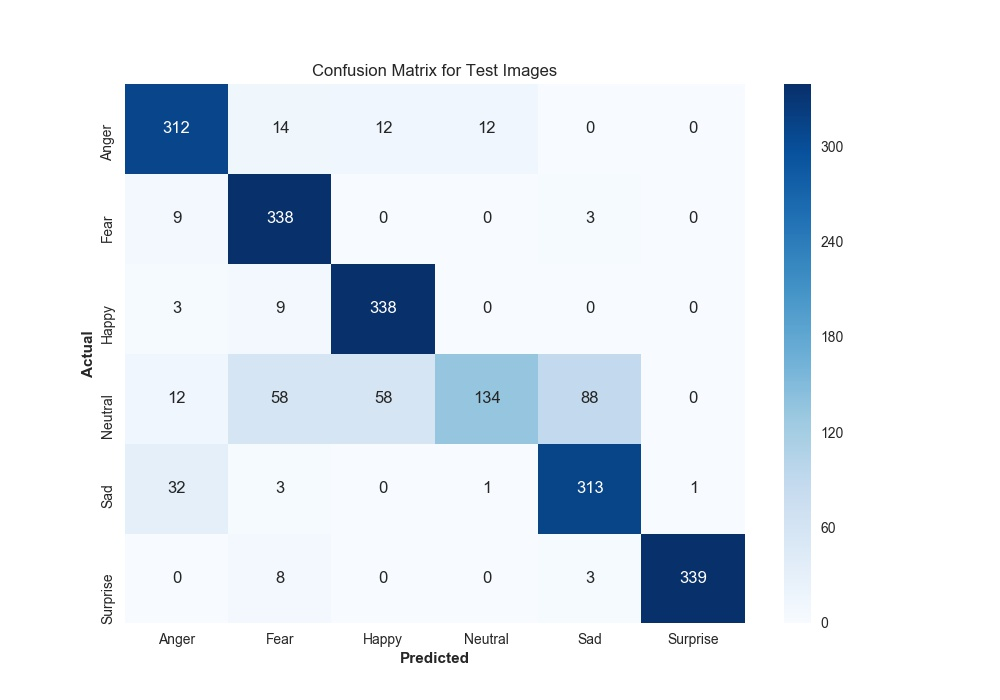
\includegraphics[keepaspectratio=true,scale=0.5]{__resources/Results/confusion.jpg}
		\caption{Confusion Matrix Heatmap}
		\label{conf}
	\end{center}
\end{figure}
\newpage

From this confusion matrix we are able to plot out a number of performance metrics besides the basic training accuracy and loss. Firsly, the recall of each is measured. The recall of a class can be described are the number of true positives divided by the number of true positives and false negatives, as seen in equation 6.2.1. 

\begin{equation}\label{eq:recall}
Recall = 
\frac{
True positive
}{
True Positive + False Negative
}
\end{equation}

Also, the precision of model can be calculated. The precision is a measure of the the number of true positives classified divided by the sum of true positives and false positives, which can be seen in equation 6.2.2

\begin{equation}\label{eq:recall}
Precision = 
\frac{
	True positive
}{
	True Positive + False Positive
}
\end{equation}

From these equations, and using the results found in the confusion matrix, the table below displays the performance of the model. See 
Table \ref{table:per} for further insight into the results.

\begin{table}[ht]
	\begin{center}
	\begin{tabular}{|p{5cm}||p{2cm}||p{2cm}|}		
		\hline
		
		\multicolumn{3}{|c|}{Testing Performance Measures} \\
		\hline
		\textbf{Class}& \textbf{Precision} &  \textbf{Recall}\\
		\hline
		Anger  & 84.7\% & 89.14\%	\\
		\hline
		Fear  & 78.6\% & 96.5\%	\\
		\hline
		Happy  & 82.8\% & 96.5\%  \\
		\hline
		Neutral & 91.15\% & 38.2\%	\\
		\hline	
		Sadness &  76.9\% & 89.4\%	\\
		\hline
		Surprise & 99.7 \% & 96.8\%	\\
		\hline	
		\hline 
		\textit{Accuracy} & \multicolumn{2}{|c|}{ 84.47\%} \\
		\hline
		\textit{Average Precision} & \multicolumn{2}{|c|}{ 85.64\%} \\
		\hline
		\textit{Average Recall} & \multicolumn{2}{|c|}{ 84.42\%} \\
		\hline
	\end{tabular}
	\caption{Table of Performance Measure Results}
	\label{table:per}
	\end{center}
\end{table}
	
\section{Testing Model with New Data}
Single inference was performed with images taken from google so see how well the model performed without any of the preprocessing steps. One image was chosen at random for each emotion. From the results seen in Figure \ref{inf}.

\begin{figure}[ht]
	\begin{center}
		\advance\leftskip-3cm
		\advance\rightskip-3cm
		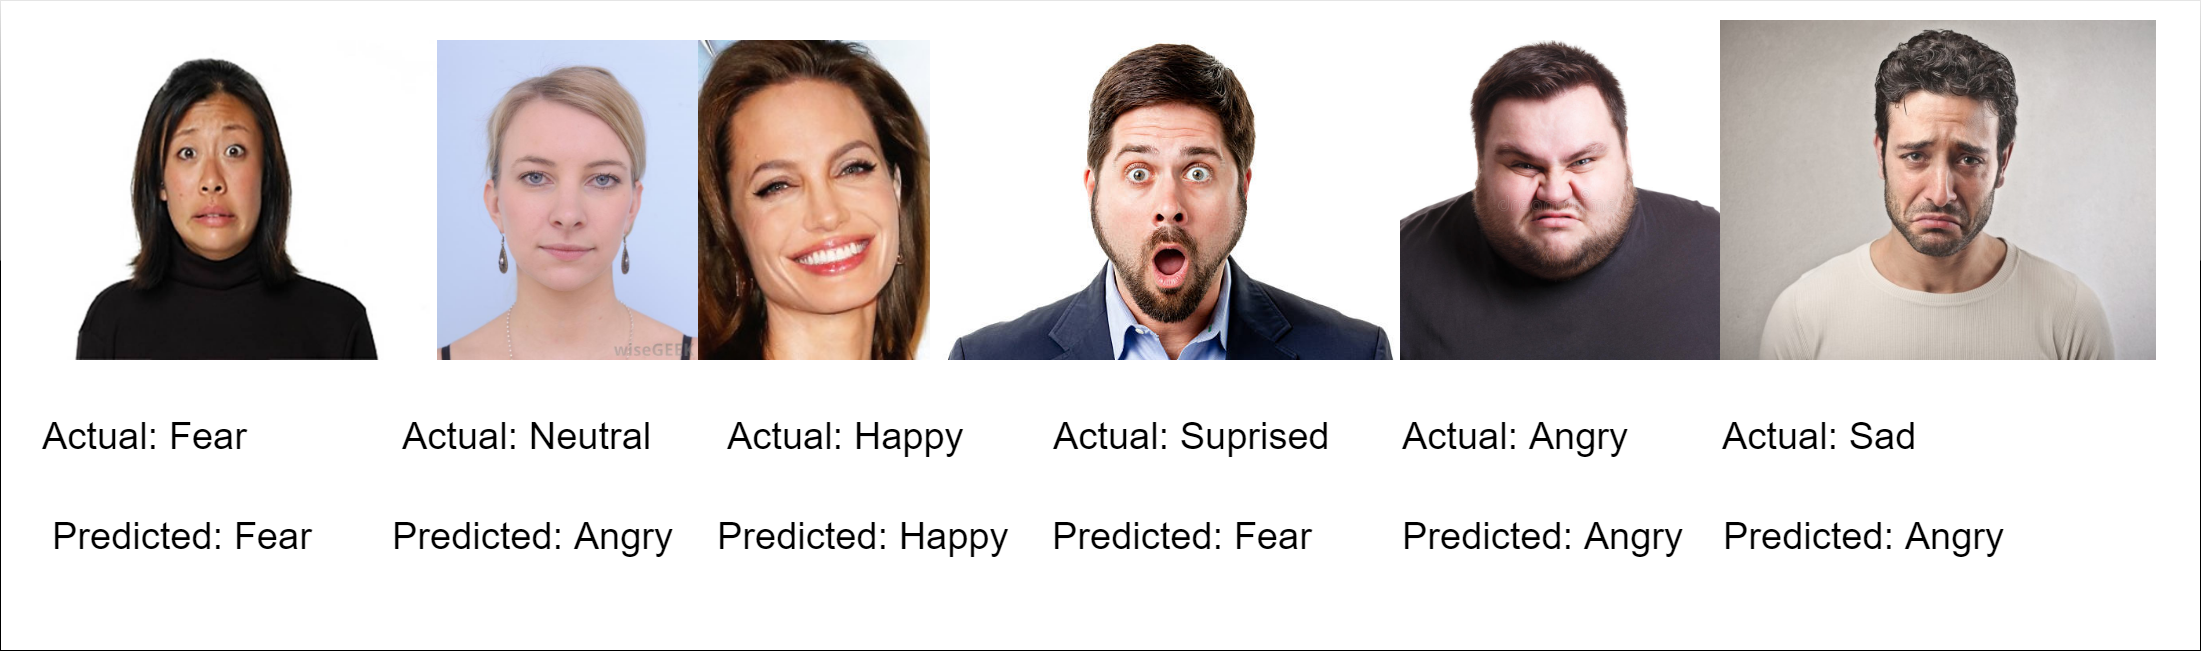
\includegraphics[keepaspectratio=true,scale=0.25]{__resources/Testing/inference.png}
		\caption{Single Predictions on Non-preprocessed Images}
		\label{inf}
	\end{center}
\end{figure}


\section{Concluding Remarks of Testing and Evaluation}
In conclusion, the training performance evaluation was discussed in regards to the loss and accuracy of the model during the training stage. Testing was done on the trained model with 350 images per class with a highly correct classification score excluding the neutral class. Recall and precision scores were calculated using the a confusion matrix. Lastly, single inference was performed using randomly selected images sourced from Google images in order to examine how the model performed.

The neutral class did not have as high of an accurate classification score as the rest of the classes. A speculated reason for this might be because the facial features of the subject may just naturally appear like other facial features, such as sadness, which was classified 88 times out of 350. Also, it is possible that by the augmented images for this class may have morphed too much, therefore making them appear to look like another class (happy or sad in this case).
In terms of the single predictions performed, Although these classifications were only moderately accurate (classifying 3/6 images correctly),  it should be noted that facial cropping needs to be performed on each image for more accurate results.


